\subsection{Abstraction and Automation}
  \noindent
  \marginnote{3.4.1.1}Problem solving is the process of finding solutions to a certain problem. One of the main tools used when problem solving is the application of Logical Reasoning which is the process of using a given set of facts to determine whether new facts are true or false. To solve a problem another important step is to identify what the problem is.\\
  \marginnote{3.4.1.2}An Algorithm is a sequence of steps that can be followed to complete a task and that always terminate. An example of an algorithm (written in pseudo-code) is as follows:
  \begin{python}
func bubblesort( var a as array )
for i from 1 to N
	for j from 0 to N - 1
	  if a[j] > a[j + 1]
	    swap( a[j], a[j + 1] )
end func
  \end{python}
  We can use a technique called hand-tracing/ dry running to work through the code and see if it works as intended. An example of a dry run is as follows:
  \begin{table}[H]
    \centering
    \begin{tabular}{| C{2cm} | C{2cm} | C{2cm} C{2cm} C{2cm} C{2cm} |}
      \hline
      \textbf{i} & \textbf{j} & \multicolumn{4}{c|}{\textbf{a}} \\
      \hline
      0 & 0 & 3 & 2 & 1 & 4 \\
      \cline{3-6}
      1 & 0 & 2 & 3 & 1 & 4 \\
      \cline{3-6}
      1 & 1 & 2 & 1 & 3 & 4 \\
      \cline{3-6}
      1 & 2 & 2 & 1 & 3 & 4 \\
      \cline{3-6}
      2 & 0 & 1 & 2 & 3 & 4 \\
      \cline{3-6}
      2 & 1 & 1 & 2 & 3 & 4 \\
      \cline{3-6}
      2 & 2 & 1 & 2 & 3 & 4 \\
      \cline{3-6}
      3 & 0 & 1 & 2 & 3 & 4 \\
      \cline{3-6}
      3 & 1 & 1 & 2 & 3 & 4 \\
      \cline{3-6}
      3 & 2 & 1 & 2 & 3 & 4 \\
      \hline
    \end{tabular}
  \end{table}
  \noindent
  This shows what happens to the data throughout the process at which the algorithm is being run.\\
  \marginnote{3.4.1.3}The main concept behind abstraction is to reduce a problem to its most basic parts, its essential features. This is useful as it allows a programmer to solve the problem without having to fuss too much about the details, abstraction is also useful because it allows the solution to one problem to be implemented in other similar problems. In general, there are two main types of abstraction:
  \begin{itemize}
    \setlength{\itemsep}{0em}
    \item Representational Abstraction
    \begin{itemize}
      \setlength{\itemsep}{0em}
      \item This is the process of removing unnecessary details so that only information that is required to solve the problem remains. An example of this is a train map, as this shows how the different stations are connected, but doesn't really care about actual distance or time taken.
    \end{itemize}
    \item Abstraction by generalisation/categorisation
    \begin{itemize}
      \setlength{\itemsep}{0em}
      \item This is the concept of reducing problems by putting aspects of a problem into hierarchical categories using an "is a kind of" relationship. An example of this is could be a tree showing the different sciences, e.g:
    \end{itemize}
  \end{itemize}
  \begin{center}
    \begin{tikzpicture}[
    level 1/.append style={level distance=2cm},
    level 2/.append style={level distance=2cm}]
    \tikzstyle{every node}=[rectangle, rounded corners, minimum width=2cm, minimum height=1cm,text centered, draw=black]
    \Tree
    [.Science
      [.{Mathematics}
          [.{Applied Mathematics}	]
          [.{Pure Mathematics} ]
      ]
      [.{Physics} ]
      [.{Chemistry} ]
      [.{Biology} ]
    ]
    \end{tikzpicture}
  \end{center}
  \marginnote{3.4.1.4}The process of information hiding involves hiding all details about an object that do not contribute to its essential characteristics. A simple example of this is using a car, as you can control it by using the steering wheel, gearbox, pedals, etc. and don't need to know the mechanics behind it.\\
  There are many different types of abstractions, for example:
  \begin{itemize}
    \setlength{\itemsep}{0em}
    \item \marginnote{3.4.1.5}Procedural Abstraction
    \subitem This is the concept that all solutions can be broken down into a series of procedures, an example would be a recipe.
    \item \marginnote{3.4.1.6}Functional Abstraction
    \subitem This is the concept that all solutions can be broken down into reusable functions. Functions can be thought of as abstracted procedures as one can call a function without completely knows how it works.
    \item \marginnote{3.4.1.7}Data Abstraction
    \subitem This is the concept of hiding how a data type is represented, making it easier to construct new data objects (called compound data objects). It also involves separating implementations of data objects and the user interface.
    \item \marginnote{3.4.1.8}Problem Abstraction/ Reduction
    \subitem This is the process of removing unnecessary details in a problem until the underlying problem is identified to see if this is the same as a problem that has already been solved.
  \end{itemize}
  \marginnote{3.4.1.9}Decomposition is the process of breaking a large task into a series of subtasks. Procedural decomposition is the process of breaking down a task into procedures and subroutines.\\
  \marginnote{3.4.1.10}Composition is the building up of a whole system from smaller units. The opposite of decomposition. This involves:
  \begin{itemize}
    \setlength{\itemsep}{0em}
    \item Writing all the procedures and linking them together to create compound procedures.
    \item Creating data structures and combining them to form compound structures.
  \end{itemize}
  \begin{center}
    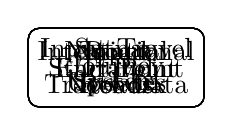
\begin{tikzpicture}[
    level 1/.append style={level distance=2cm},
    level 2/.append style={level distance=2cm}]
    \tikzstyle{every node}=[rectangle, rounded corners, text width=2cm,  minimum width=2cm, minimum height=1cm,text centered, draw=black]
    \Tree
    [.\node[anchor=north west](a){Satnav System};
      [.\node[anchor=north west](b){Journey};
        [.\node[anchor=north west](c){Start Point};	]
        [.\node[anchor=north west](d){End Point}; ]
      ]
      [.\node[anchor=north west](e){Travel};
        [.\node[anchor=north west](f){Input Travel Data};	]
        [.\node[anchor=north west](g){Input Travel Updates}; ]
      ]
      [.\node[anchor=north west](h){Road Network};
        [.\node[anchor=north west](i){National Roads};	]
        [.\node[anchor=north west](j){International Roads}; ]
      ]
    ]
    %\node(k)[below=6cm]{Calculate Route};
    %\draw (c.south) -| (k);
    %\draw (d.south) -| (k);
    %\draw (f.south) -| (k);
    %\draw (g.south) -| (k);
    %\draw (i.south) -| (k);
    %\draw (j.south) -| (k);
    \end{tikzpicture}
  \end{center}
  \marginnote{3.4.1.11}Automation is the process of creating computer models (abstraction of real world objects/ phenomena) of real-life situations and putting them into action to solve problems. This is done by:
  \begin{itemize}
    \setlength{\itemsep}{0em}
    \item Understanding the problem.
    \item Creating Algorithm.
    \item Implementing the algorithms in program code.
    \item Implementing the models in data structures.
    \item Executing the code.
  \end{itemize}
\subsection{Regular Languages}
  \noindent
  \marginnote{3.4.2.1}A finite state machine is any device device that stores its current state and whose status can change as the result of an input. Mainly used as a conceptual model for designing and describing systems. A state transition diagram is a visual representation of an FSM using circles and arrows, whereas a state transition table is a tabular representation of an FSM showing input, current state, and next state. Within a state transition diagram, there may be an accepting state, represented by two concentric circles, which shows whether an input has been accepted. An FSM doesn't necessarily need an accepting state. Below is an example of both a State Transition Diagram and a state transition table.\\
  \begin{figure}[H]
    \centering
    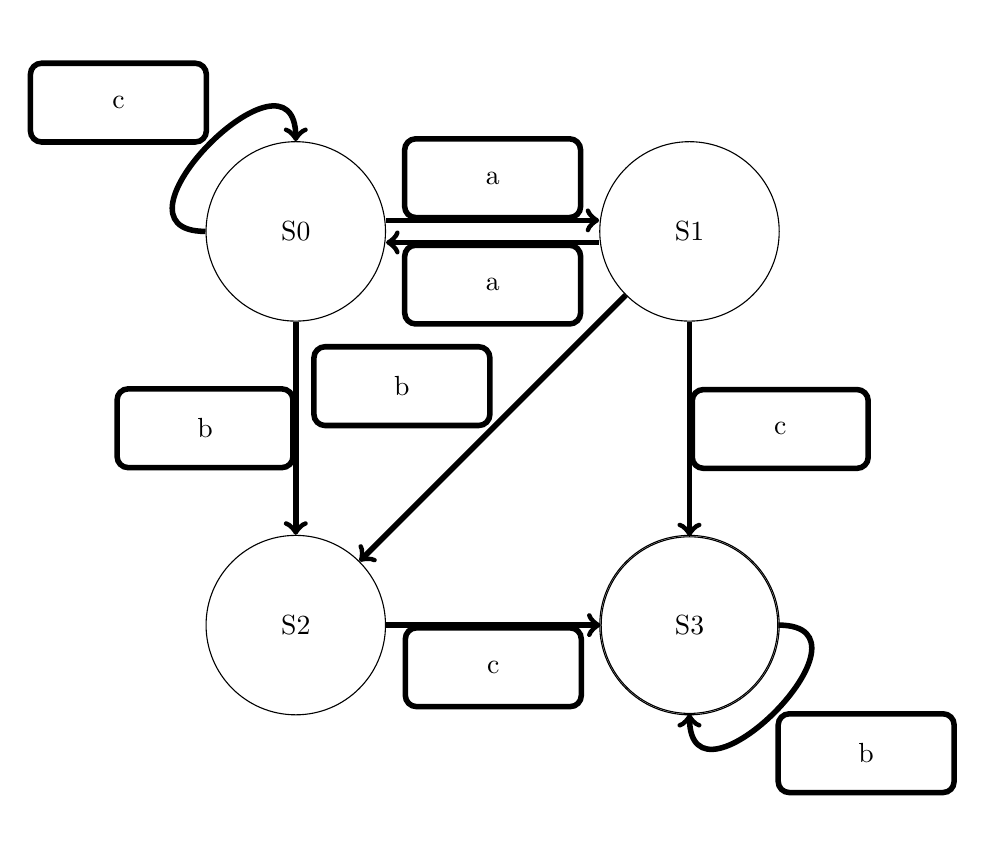
\begin{tikzpicture}
      \def \n {5};
      \node[circle, minimum width=1cm, draw=black](S0) at (0,\n) {S0};
      \node[circle, minimum width=1cm, draw=black](S1) at (\n,\n) {S1};
      \node[circle, minimum width=1cm, draw=black](S2) at (0,0) {S2};
      \node[circle, minimum width=1cm, draw=black](S3) at (\n,0) {S3};
      \node[circle, minimum width=1.2cm, draw=black](S4) at (\n,0) {};

      \draw[->, line width=2pt] ([yshift= 4pt]S0.east) -- node[above] {a} ([yshift= 4pt]S1.west);
      \draw[->, line width=2pt] (S0.south) -- node[left] {b} (S2.north);
      \draw[->, line width=2pt] ([yshift= -4pt]S1.west) -- node[below] {a} ([yshift= -4pt]S0.east);
      \draw[->, line width=2pt] (S1.south west) -- node[above left] {b} (S2.north east) ;
      \draw[->, line width=2pt] (S1.south) -- node[right] {c} (S4.north);
      \draw[->, line width=2pt] (S2.east) -- node[below] {c} (S4.west);
      \draw[->, line width=2pt] (S4.east) .. controls ([xshift= 40pt]S4.east) and ([yshift= -40pt]S4.south) .. node[below right] {b} (S4.south);
      \draw[->, line width=2pt] (S0.west) .. controls ([xshift= -40pt]S0.west) and ([yshift= 40pt]S0.north) .. node[above left] {c} (S0.north);
    \end{tikzpicture}
    \caption*{State Transition Diagram}
  \end{figure}
  \begin{figure}[H]
    \centering
    \begin{tabular}{| C{4cm} | C{4cm} | C{4cm} |}
      \hline
      Input & Current State & Next State \\
      \hline
      c & S0 & S0 \\
      a & S0 & S1 \\
      b & S0 & S2 \\
      a & S1 & S0 \\
      b & S1 & S2 \\
      c & S1 & S3 \\
      c & S2 & S3 \\
      b & S3 & S3 \\
      \hline
    \end{tabular}
    \caption*{State Transition Table}
  \end{figure}
  A Mealy Machine is a type of finite state machine which also produces an output, this output can be shown on a diagram by instead of labelling each transition with ``input'', you label them with ``input/output'', and that output is outputted when the transition it is on occurs. This can also be represented in a state transition Table by simply adding a column.
  
  \noindent
  \marginnote{4.4.2.2}Maths for Regular Expressions
  
  \noindent
  \marginnote{4.4.2.3}Regular Expressions
  
  \noindent
  \marginnote{4.4.2.4}Regular Languages
  
\subsection{Context-free Languages}
  
  \noindent
  \marginnote{4.4.3.1}Backus-Naur Form(BNF)/Syntax Diagrams
  
\subsection{Classification of Algorithms}
  
  \noindent
  \marginnote{4.4.4.1}Comparing algorithms
  
  \noindent
  \marginnote{4.4.4.2}Maths For Understanding Big-O Notation
  
  \noindent
  \marginnote{4.4.4.3}Order of Complexity
  
  \noindent
  \marginnote{4.4.4.4}Limits of Computation
  
  \noindent
  \marginnote{4.4.4.5}Classification of Algorithmic Problems
  
  \noindent
  \marginnote{4.4.4.6}Computable and non-computable problems
  
  \noindent
  \marginnote{4.4.4.7}Halting Problem

\subsection{A model of computation}
  \noindent
  \marginnote{4.4.5.1}Turing Machine